% Document class report-template accepts either: project-plan or final-report option
\documentclass[final-report]{report-template}

% Packages I want to use in my report.
\usepackage{graphicx}
\usepackage{subfigure}
\usepackage{amsmath}
\usepackage{blindtext}
\usepackage{listings}
\usepackage{lmodern}
\usepackage{multirow}
\usepackage{appendix}
\usepackage{algorithm}
\usepackage{algpseudocode}

% \def\LOGO{%
% \begin{picture}(0,0)\unitlength=1cm
% \put (3,-1) {\includegraphics[width=5em]{school_badge.png}}
% \end{picture}
% }

% Define and Set the code part style
\lstdefinestyle{mystyle}{
    backgroundcolor=\color{backcolour},   
    commentstyle=\color{blue!20!black!50!green},
    keywordstyle=\color{blue!70},
    numberstyle=\tiny\color{codegray},
    stringstyle=\color{codepurple},
    basicstyle=\footnotesize,
    breakatwhitespace=false,         
    breaklines=true,                 
    captionpos=b,                    
    keepspaces=true,                 
    numbers=left,                    
    numbersep=5pt,                  
    showspaces=false,                
    showstringspaces=false,
    showtabs=false,                  
    tabsize=2
}
\lstset{style=mystyle, escapeinside=``}


% Directory where I save my figures.
\graphicspath{{./figures/}}

% \university{Imperial College London}
% \department{Department of Earth Science and Engineering}
% \course{MSc in Applied Computational Science and Engineering}
% \title{Forecasting induced seismicity in Oklahoma}
% \author{Zhiyong Liu}
% \email{zl1220@ic.ac.uk}
% \githubusername{acse-liuzyon}
% \supervisors{Dr. Stephen P. Hicks}
\repository{https://github.com/acse-2020/acse2020-acse9-finalreport-liuzyon}


\begin{document}

\begin{titlepage}

\newcommand{\HRule}{\rule{\linewidth}{0.5mm}} % Defines a new command for the horizontal lines, change thickness here

\center % Center everything on the page

%----------------------------------------------------------------------------------------
%	HEADING SECTIONS
%----------------------------------------------------------------------------------------

\textsc{\LARGE Imperial College London}\\[1.5cm] % Name of your university/college
\textsc{\Large Department of Earth Science and Engineering}\\[0.5cm] % Major heading such as course name
\textsc{\large MSc in Applied Computational Science and Engineering}\\[0.5cm] % Minor heading such as course title

%----------------------------------------------------------------------------------------
%	TITLE SECTION
%----------------------------------------------------------------------------------------

\HRule \\[0.4cm]
{ \huge \bfseries Forecasting induced seismicity in Oklahoma}\\[0.4cm] % Title of your document
\HRule \\[1.5cm]
%----------------------------------------------------------------------------------------
%	AUTHOR SECTION
%----------------------------------------------------------------------------------------

\begin{minipage}{0.4\textwidth}
    \begin{flushleft} \large
    \emph{Author:}\\
    Zhiyong \textsc{Liu}\\ % Your name
    zl1220@ic.ac.uk\\
    Github: acse-liuzyon
    \end{flushleft}
    \end{minipage}
    ~
    \begin{minipage}{0.4\textwidth}
    \begin{flushright} \large
    \emph{Supervisor:} \\
    Dr. Stephen P. \textsc{Hicks}\\ % Supervisor's Name
    s.hicks@imperial.ac.uk
    \end{flushright}
\end{minipage}\\[2cm]

%----------------------------------------------------------------------------------------
%	LOGO SECTION
%----------------------------------------------------------------------------------------


\includegraphics[width=0.3\textwidth]{school.png}\\[3cm] % Include a department/university logo - this will require the graphicx package
 
%----------------------------------------------------------------------------------------


%----------------------------------------------------------------------------------------
%	DATE SECTION
%----------------------------------------------------------------------------------------

{\large \today}\\[1cm] % Date, change the \today to a set date if you want to be precise

\githubrepo  % GitHub repository
\vfill % Fill the rest of the page with whitespace

\end{titlepage}


% Metadata used for the title page.

\tableofcontents
\newpage

% Abstract
\section*{Abstract}
\addcontentsline{toc}{section}{Abstract}
Human activities can cause minor earthquakes, which changes the stresses and strains on the earth's crust.
These earthquakes are called induced earthquakes and most have a low magnitude. 
Multi-year research by the United States Geological Survey (USGS) published in 2015 showed that most of large earthquakes occured in Oklahoma may have been caused by deep injection of wastewater from the oil industry.
In this project, a unique and rich dataset of industrial activities from regions in Oklahoma are used and correlations between these activities and seismicity are confirmed.
With existing high-quality earthquake catalogues in these regions, possible signatures of human-induced seismicity are retrospectively forecasted through machine learning techniques. 
At the end of the project, a working forecasting model is generated and tested the permormance by the test dataset splitted from total dataset.

\textbf{Key Words:} induced earthquakes, machine learning method, forecasting model
\newpage

% Introduction section
\section{Introduction}
It is well known that humans can cause earthquakes through fluid injection and extraction. Ellsworth stated the understanding of the causes and mechanics of human-induced earthquakes. It includes wastewater injection, emerging oil and gas recovery technologies, and other indirect induced activities,
including deep fluid injection \citep{ellsworth2013injection}.
Norbeck and Rubinstein genreated a model based on fluid flow and seismic physics, which associate the past injection trends with the seismicity patterns \citep{norbeck2018hydromechanical}.
Such cases of induced seismicity have been recorded and proven in Oklahoma, where seismicity has been increased dramatically since 2010.
In cases like Oklahoma, because the rate of earthquakes was very low before high-rate wastewater injection, it is relatively easy to determine the fundamental causes of induced seismicity.
Therefore, due to the low background stress in intraplate regions, the human triggering signatures are clearly identifiable.
However, in tectonically-active areas, it is more challenging to distinfuish between natural and triggered seismicity.
In tectonically active regions in the US, such as California, although oil and gas extraction has taken place for many decades, only a handful of studies have been published with a focus on these areas \citep{Hough2017WasTM}. 
Big-data and statistical approaches will be crucial in separating natural causes from potential human triggering factors in these areas.
In regions from Oklahoma, Hincks et al. developed a Bayesian network to for quantitative evaulation of correlations between well operational parameters, geological formation, and seismicity.
The injection depth relative to crystalline basement was found to be the most significant parameter for seismic moment release \citep{hincks2018oklahoma}.
Also, Wozniakowska and Eaton performed a machine learning estimation of the seismogenic activation potential for each well using logistic regression and also found that the injection depth influence greatly the seismogenic activation potential \citep{wozniakowska2020machine}.

The correlations of induced earthquakes with fluid injection activities are well established, even in previous research some physics models are also developed for earthquake prediction.
It is still not known why some areas are more susceptible to induced earthquakes.
In this project, Several unique and rich datasets of industrial activities from regions in Oklahoma are used to statistically evaluate and retropectively forecast possible signatures of human-induced seismicity from existing high-quality earthquake in these regions. 
These datasets contains geological formation, injections, hydraulic fracturing activities and wells, which all have millions of items.
They were selected subset from 2011 to 2018 and displayed on the local map of Oklahoma. Rough visual correlations between the earthquakes and these potential induced factors were discovered.
Then, stepwise regression method was used to choose statistically significant features from all features. A logistic model was fitted before and after stepwise regression, which proved that the work of features selection indeed benefit to induced forecasting. 

In previous studies for induced earthquakes in Oklahoma, forecasting works were almost always implemented using regression models. Compared to them, after selecting statistically significant features, this project originally designed and implemented a neural network for induced seismicity forecasting, which effectively improves the performance of model fitting and prediction. 

% Another section
\section{Software Description}
\subsection{Visualization: Matplotlib \& GeoPandas}
GeoPandas can help researcher make working with geospatial data in Python easier. It extends the datatypes in Pandas, which allows users perform spatial operations on geometric types.
Matplotlib is a comprehensive library for creating static, animated, and interactive visualizations in Python.
Combining these two libraries, after setting the appropriate coordinate system, the data items can be mapped in spatial clearly by short code.
Figure~\ref{fig:earthquake_plot} shows all earthquakes recorded in the dataset. The red rectangule is the interest area to study for this project.
Here we only concentrate on the earthquakes which have a magnitude greater than 2.0.
\begin{figure}
    \begin{center}
        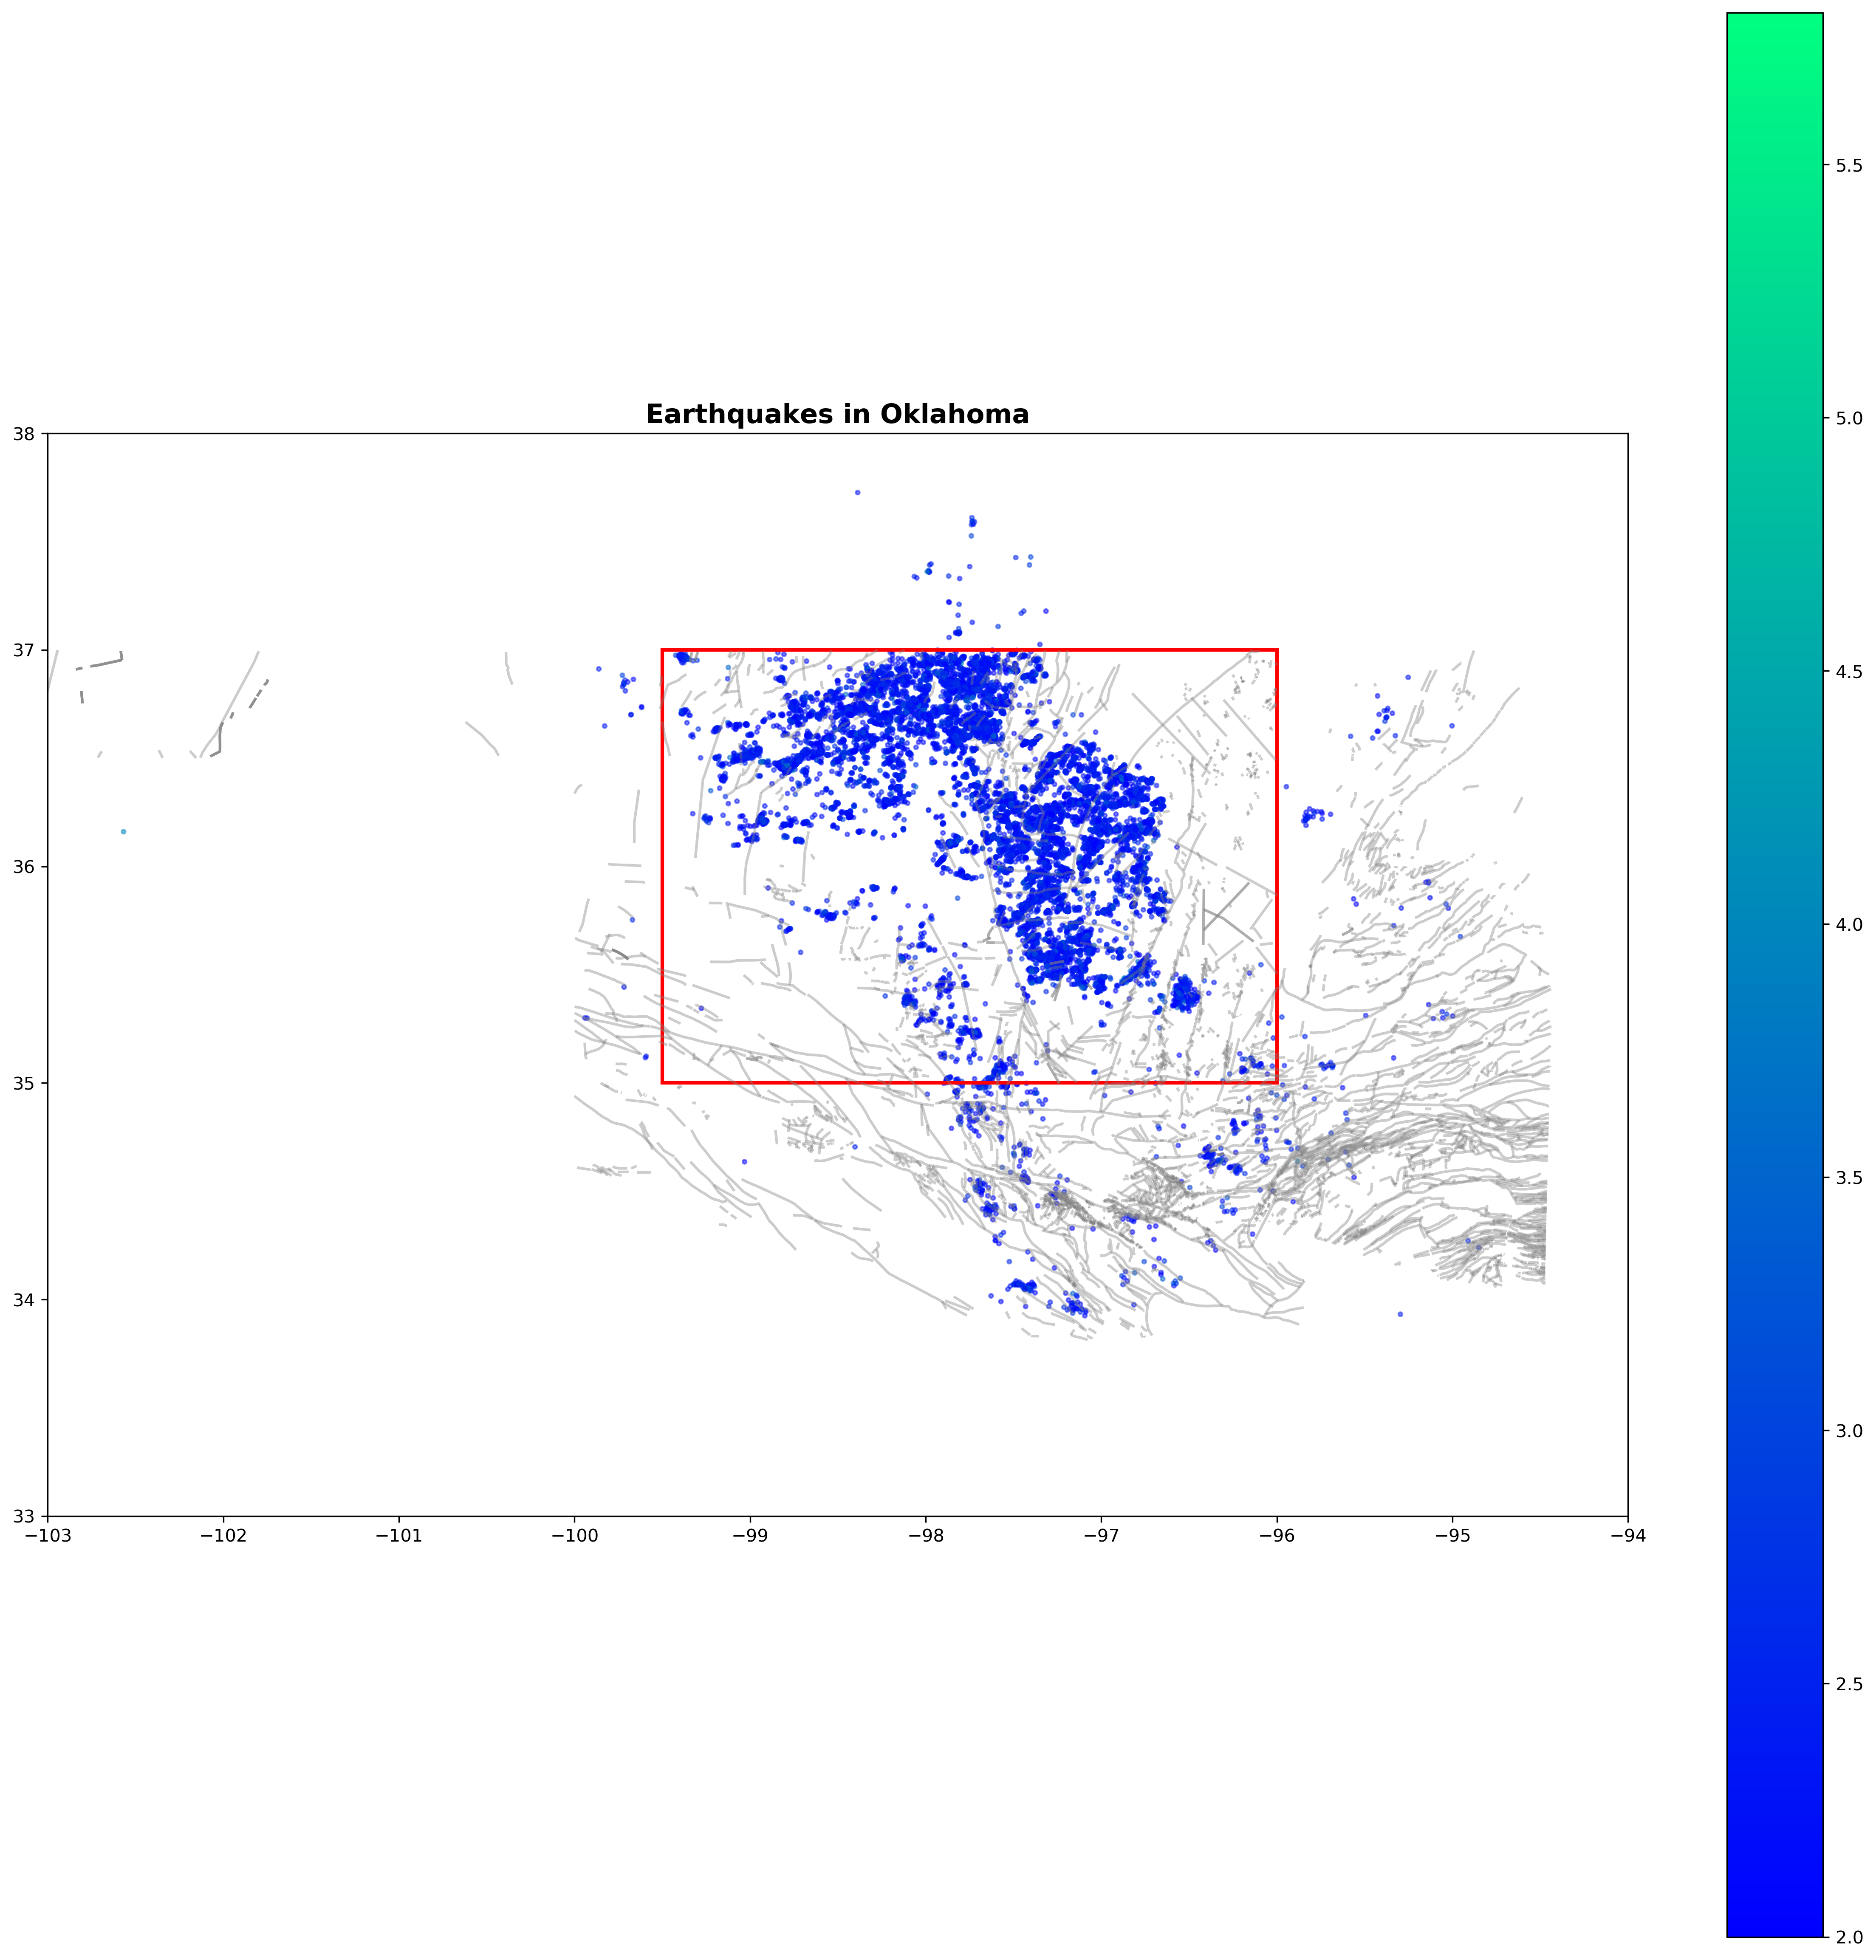
\includegraphics[width=0.8\textwidth]{earthquake_plot.png}
    \end{center}
    \caption{\label{fig:earthquake_plot} Earthquake Occurrences in Oklahoma.}
\end{figure}

\subsection{Stepwise Regression}
\label{sec:stepwise}
In any phenomenon, some factors will play a more important role in determining the outcome. Stepwise Regression is method which is widely used to find which factors are important and which are not. 
The factors that have a rather high p-value do not make a meaningful contribution to the accuracy of our predictions. 
Therefore, only the important factors are retained to ensure that the model make predictions based on the factors that will help it produce the most accurate results.

P-values are often used to see if the patterns they measured were statistically significant. If the p-value of a statistical test is small enough, we are able to reject the null hpytothesis of the test and the pattern measured is statistically significant.
The most common threshold for p is 0.05. For the variable whose p-value is greater than 0.05, we can assume that it is not statistically significant as shown in Fig~\ref{fig:p-value}. Here is step in stepwise logistic regression process.
The `injection\_vol', `HF\_Base\_Water\_Volume', `HF\_Base\_NoWater\_Volume' both have a p-value than threshold 0.05 in logistic regression results, which are not statistically significant and should be eliminated in later process.

In the process of regression analysis, there usually exists the problem of high collinearity, which can cause the following influence:
\begin{itemize}
    \item The model parameters are estimated inaccurately, and sometimes even the sign of the regression coefficients is exactly opposite to the actual situation, for example, the characteristic coefficients that should logically have positive coefficients are calculated to be negative.
    \item The independent variables that should be significant are not significant, and the independent variables that are not significant show the significance.
\end{itemize}

VIF.(required continue)


\begin{algorithm}
    \caption{An algorithm with caption}\label{alg:cap}
    \begin{algorithmic}
    \Require $n \geq 0$
    \Ensure $y = x^n$
    \State $y \gets 1$
    \State $X \gets x$
    \State $N \gets n$
    \While{$N \neq 0$}
    \If{$N$ is even}
        \State $X \gets X \times X$
        \State $N \gets \frac{N}{2}$  \Comment{This is a comment}
    \ElsIf{$N$ is odd}
        \State $y \gets y \times X$
        \State $N \gets N - 1$
    \EndIf
    \EndWhile
    \end{algorithmic}
    \end{algorithm}

In this project, we performed a stepwise logistic regression that used a forward selection approach on all interest potential factors \citep{Ryan}.
All features were initially excluded and a feature is added in each step whilst keping current features satisfy p-value \textless 0.05. 
This process continued untill all features kept are statistically significant. Meanwhile, in each step, we also remains the VIF \textless 10 for current kept features even some new added feature required to be eliminated.

\subsection{Neural Network Construction: Pytorch}
Pytorch is an open source machine learning library for Python and is completely based on Torch library,
used for applications such as computer vision and natural language processing. It is mostly developed by Facebook's AI Research lab (FAIR) \citep{patel2018two}. 
PyTorch provides two features:
\begin{itemize}
    \item Tensor computing (like Numpy) with strong acceleration via graphics processing units (GPU)
    \item Deep neural networks built on a type-based automatic differentiation system.
  \end{itemize}
Pytorch provides a class called Tensor (torch.Tensor) to store and operate on homogeneous multidimensional rectangular arrays of numbers. 
They are tailored for datasets in machine learning. Tensors in Pytorch are similar to Numpy Arrays, but it supports to be operated on a CUDA-capable Nvidia GPU \citep{paszke2019pytorch}.

To define a neural network in Pytorch, it is pretty convenient to create a class that inherits from nn.Module as below:
\begin{lstlisting}[language=Python]
    # Get cpu or gpu device for training.
    device = "cuda" if torch.cuda.is_available() else "cpu"
    print("Using {} device".format(device))
    
    # Define model
    class NeuralNetwork(nn.Module):
        def __init__(self):
            super(NeuralNetwork, self).__init__()
            self.flatten = nn.Flatten()
            self.linear_relu_stack = nn.Sequential(
                nn.Linear(4, 8),
                nn.ReLU(),
                nn.Linear(8, 8),
                nn.ReLU(),
                nn.Linear(8, 2),
                nn.ReLU()
            )
    
        def forward(self, x):
            x = self.flatten(x)
            logits = self.linear_relu_stack(x)
            return logits
    
    model = NeuralNetwork().to(device)
\end{lstlisting}
User can define the layers of the network in the \textit{\_\_init\_\_} function and indicates how data will pass through the network in the \textit{forward} function. 
With Pytorch, user can move it to the GPU to accelate operations in the neural netwok if available. Figure~\ref{fig:neural_network_example} is the model created above trained on the playground online through Tensorflow. 
The neural network prediction model used in this project is implemented by this way.

\subsection{Feature Attribution: Captum}
Feature attribution is the technique to investgiate how much each feature in the model contributes to the prediction for given dataset fitting. 
With the increase in model complexity and the resulting lack of transparency, model interpretability methods have become increasingly important in machine learning field.
In this project, we implemented a neural network model with the PyTorch library \citep{PyTorch} for improving the accuracy of prediction. Therefore, we use the Captum for feature attribution in neural network model, which is a model interpretability and understanding library for Pytorch.
It includes general purpose implementations of integrated gradients, saliency maps, smoothgrad, vargrad and others for PyTorch models.

Captum provides advanced algorithms, including Intergarated gradientes used in this project, to provides users an simple way to understand which features are contributing to a models' output.
Integrated gradients represents the integral of gradients with respect to inputs along the path from a given baseline to input. The integral can be approximated using a Riemann Sum or Gauss Legendre quadrature rule. Formally, it can be described as follows in Equation \eqref{equ:inreGrad}:

\begin{equation}
    IntegratedGrads_{i}(x) ::= (x_{i} - x_{i}^{'}) \times 	\int_{\alpha=0}^1 \frac{\partial F(x^{'}+\alpha \times (x-x^{'}))}{\partial x_{i}} d\alpha  \label{equ:inreGrad}    
\end{equation}

Intergarated Gradients along the i-th dimension of input X. Alpha is the scaling coffecient \citep{sundararajan2017axiomatic}.

As shown in Fig~\ref{fig:feature_importance}, this is the result of feature importance analysis for the model trained in official tutorial of Captum.
The official tutorial used an example model trained on the titanic survival data. 
It first trained a deep neural network on the data using Pytorch and used Captum to understand which of the features were most important and how the network reached its prediction.
The features involved Age, Sibsp, Parch, Fare, Gender, Embark, Class and the target is a binary indicating whether passager is survived. After normalization and one-hot encodings, the neural network architecture was defined and trained. 
The neural network had a simple architecture using 2 hidden layers, the first with 12 hidden units and the second with 8 hidden units, each with Sigmoid non-linearity.
The final layer performed a softmax operation and had 2 units, corresponding to the outputs of either survived or not survived. The accuracy of this model on dataset achieved to $81.6\%$. To perform feature attribution on this model, this example applied integrated Gradients, which is one of the Feature Attribution methods included in Captum. The feature attribution method code is shown in below.

\begin{lstlisting}[language=Python]
    ig = IntegratedGradients(model)
    test_input_tensor.requires_grad_()
    attr, delta = ig.attribute(test_input_tensor,target=1, return_convergence_delta=True)
    attr = attr.detach().numpy()

    # Helper method to print importances and visualize distribution
    def visualize_importances(feature_names, importances, title="Average Feature Importances", plot=True, axis_title="Features"):
        print(title)
        for i in range(len(feature_names)):
            print(feature_names[i], ": ", '%.3f'%(importances[i]))
        x_pos = (np.arange(len(feature_names)))
        if plot:
            plt.figure(figsize=(12,6))
            plt.bar(x_pos, importances, align='center')
            plt.xticks(x_pos, feature_names, wrap=True)
            plt.xlabel(axis_title)
            plt.title(title)
    visualize_importances(feature_names, np.mean(attr, axis=0))
\end{lstlisting}

The result of feature attribution was listed in Table~\ref{tab:feature_importance} and shown in Fig~\ref{fig:feature_importance}.
From the feature attribution information, we obtain some interesting insights regarding the importance of various features. We see that the strongest features appear to be age and being male, which are negatively correlated with survival. Embarking at Queenstown and the number of parents / children appear to be less important features generally.

\begin{table}[]
    \centering
    \caption{Average Feature Importances for each feature}
    \label{tab:feature_importance}
    \resizebox{\textwidth}{6mm}{
    \begin{tabular}{|c|c|c|c|c|c|c|c|c|c|c|}
    \hline
    age    & sibsp  & parch  & fare  & male   & embark\_C & embark\_Q & embark\_S & class\_1 & class\_2 & class\_3 \\ \hline
    -0.454 & -0.119 & -0.056 & 0.175 & -0.359 & 0.086     & -0.001    & -0.082    & 0.062    & 0.021    & -0.159   \\ \hline
    \end{tabular}}
    \end{table}

\section{Code Metadata}
This project was built under macOS Catalina environment with Jupyter Notebook 6.0.3 and Python 3.7.6.
The information of libraries and their usages are listed in Table~\ref{tab:library_dependency}.

In the Github repository, source code files (\textit{.ipynb}) are stored in the src directory, including two main parts, which are feature extraction and prediction model.
The data files (\textit{.csv}) generated from feature extraction part are located at \textit{data} directory. The models (\textit{.pt}) generated from prediction part are located at the \textit{model} directory.

\begin{table}[]
    \centering
    \caption{The dependencies of this project}
    \label{tab:library_dependency}
    \begin{tabular}{|c|c|c|}
    \hline
    \textbf{Module} & \textbf{Version} & \textbf{Purpose}                                                                                                                                            \\ \hline
    os              & 3.7.11           & Search the data files (csv or xlsx) in the directory                                                                                                        \\ \hline
    numpy           & 1.18.1           & \multirow{2}{*}{Dataset process}                                                                                                                            \\ \cline{1-2}
    pandas          & 1.0.1            &                                                                                                                                                             \\ \hline
    Shapely         & 1.7.1            & \multirow{2}{*}{Map the activities on map in spatial}                                                                                                       \\ \cline{1-2}
    geopandas       & 0.9.0            &                                                                                                                                                             \\ \hline
    matplotlib      & 3.1.3            & \multirow{2}{*}{Plot the figure}                                                                                                                            \\ \cline{1-2}
    seaborn         & 0.10.0           &                                                                                                                                                             \\ \hline
    scipy           & 1.6.2            & \multirow{3}{*}{\begin{tabular}[c]{@{}c@{}}Load and process the geological formation data \\ and plot the figure\end{tabular}}                              \\ \cline{1-2}
    xarray          & 0.18.2           &                                                                                                                                                             \\ \cline{1-2}
    netCDF4         & 1.5.7            &                                                                                                                                                             \\ \hline
    statsmodels     & 0.12.2           & Used in stepwise regression                                                                                                                                 \\ \hline
    torch           & 1.9.0            & \multirow{3}{*}{\begin{tabular}[c]{@{}c@{}}Neural network model implementation and training, \\ and visualization of intermediate information\end{tabular}} \\ \cline{1-2}
    scikit-learn         & 0.22.1           &                                                                                                                                                             \\ \cline{1-2}
    livelossplot    & 0.5.4            &                                                                                                                                                             \\ \hline
    captum          & 0.4.0            & Perform the feature attribution                                                                                                                             \\ \hline
    \end{tabular}
    \end{table}

\section{Implementation}
\label{sec:Implementation}
\subsection{Data Processing and Spatial visualization}
\label{sec:dpsv}

In the initial phase of project, we imported all the available datasets (earthquake data, geological data, hydraulic fracturing data, injection data, well data) and preprocessed on various datasets. 
The metadata of earthquake dataset was exported from \textit{Oklahoma Geological Survey Earthquake Catalog Download Tool} \citep{walter2020oklahoma}.
The injection dataset was exported from \textit{Oklahoma Corporation Commission} \citep{OklahomaCorporationCommission}.
The preprocessing operations include missing values processing and data selecting by date.
The date of injection dataset we imported was in (2011, 2020). However, we only used the data between 2011 and 2018. Because the data files \textgreater 2019 supported by the \textit{Oklahoma Corporation Commission} are still under review and corrections are being made as warranted, those files are currently incomplete and subject to change.
Therefore, due to date limitation of injection data, We set the interest time in the period of 2011 to 2018 for all datasets.
For the interest area, we set it to the area whose longitude ranges in (-99.5W, -96W) and latitiude ranges in (35.0N, 37.0N), which is a available spatial scope provied by all datasets.
Then, we visualized all the selection data by \textit{matplotlib} and \textit{geopandas} module. 
The geological formation (depth to basement) is shown in Fig~\ref{fig:depth_to_basement}, and the wells along with various activities (seismicity, injection, hydraulic fracturing) are shown in Fig~\ref{fig:activity}.
The core of visualization code for all dataset is similar and is shown in the below:

\begin{lstlisting}[language=Python]
    earthquake_geometry = [Point(xy) for xy in zip(earthquake_df['longitude'], earthquake_df['latitude'])]
    earthquake_geo_df = gpd.GeoDataFrame(earthquake_df, crs = "EPSG:4326", geometry = earthquake_geometry)

    fig, ax = plt.subplots(figsize=(20, 20), dpi=300)
    oklahoma_map.plot(ax=ax, alpha=0.4,color='grey')
    earthquake_geo_df.plot(column='magnitude',ax=ax, alpha=0.5, legend=True, markersize=10)
    plt.title('Earthquake (magnitude>=2) in Oklahoma', fontsize=15,fontweight='bold')
    plt.xlim(-99.5, -96.0)
    plt.ylim(35.0, 37.0)
    plt.show()
\end{lstlisting}
The geodetic coordinate system we used for mapping in this project is 'EPSG:4326' \citep{epsg}, which is the most popular coordinate system. 

\subsection{Spatial Griding and Features Extraction}
For the interest area (longitude ranges in (-99.5W, -96W) and latitiude ranges in (35.0N, 37.0N)), we divided it into $40 \times 40$ grids. Then we counted the values of all features and target for each grid by the various data from Section~\ref{sec:dpsv}:
\begin{itemize}
    \item \textit{injection\_vol\_sum [BPD]}: The sum of injection volume in this grid.
    \item \textit{injection\_psi\_sum [PSI]}: The sum of injection pressure in this grid.
    \item \textit{injection\_depth\_avg [m]}: The mean of injection depth in this grid.
    \item \textit{injection\_under\_basement\_number [entry]}: The number of injections whose depth are deeper than the basement in this gird.
    \item \textit{active\_well\_number [entry]}: The number of working wells in this grid.
    \item \textit{well\_depth\_avg [m]}: The mean of well depth in this grid.
    \item \textit{well\_under\_basement\_number [entry]}: The number of working wells whose depth are deeper than the basement in this grid.
    \item \textit{depth\_to\_basement\_avg [m]}: The mean of the depth to the basement in this grid.
    \item \textit{hf\_number [entry]}: The number of hydraulic fracturing activities in this grid.
    \item \textit{hf\_base\_water\_volume\_sum [BPD]}: The sum of volume by hydraulic fracturing with water
    \item \textit{hf\_base\_nowater\_volume\_sum [BPD]}: The sum of volume by hydraulic fracturing with nowater
    \item \textit{earthquake\_occurrence [0 or 1]}: If earthquake occurred in this grid. 0: not occured; 1: occurred.
\end{itemize}
The data files were generated in \textit{.csv} and saved in \textit{data} directory.

\begin{figure}
    \begin{center}
        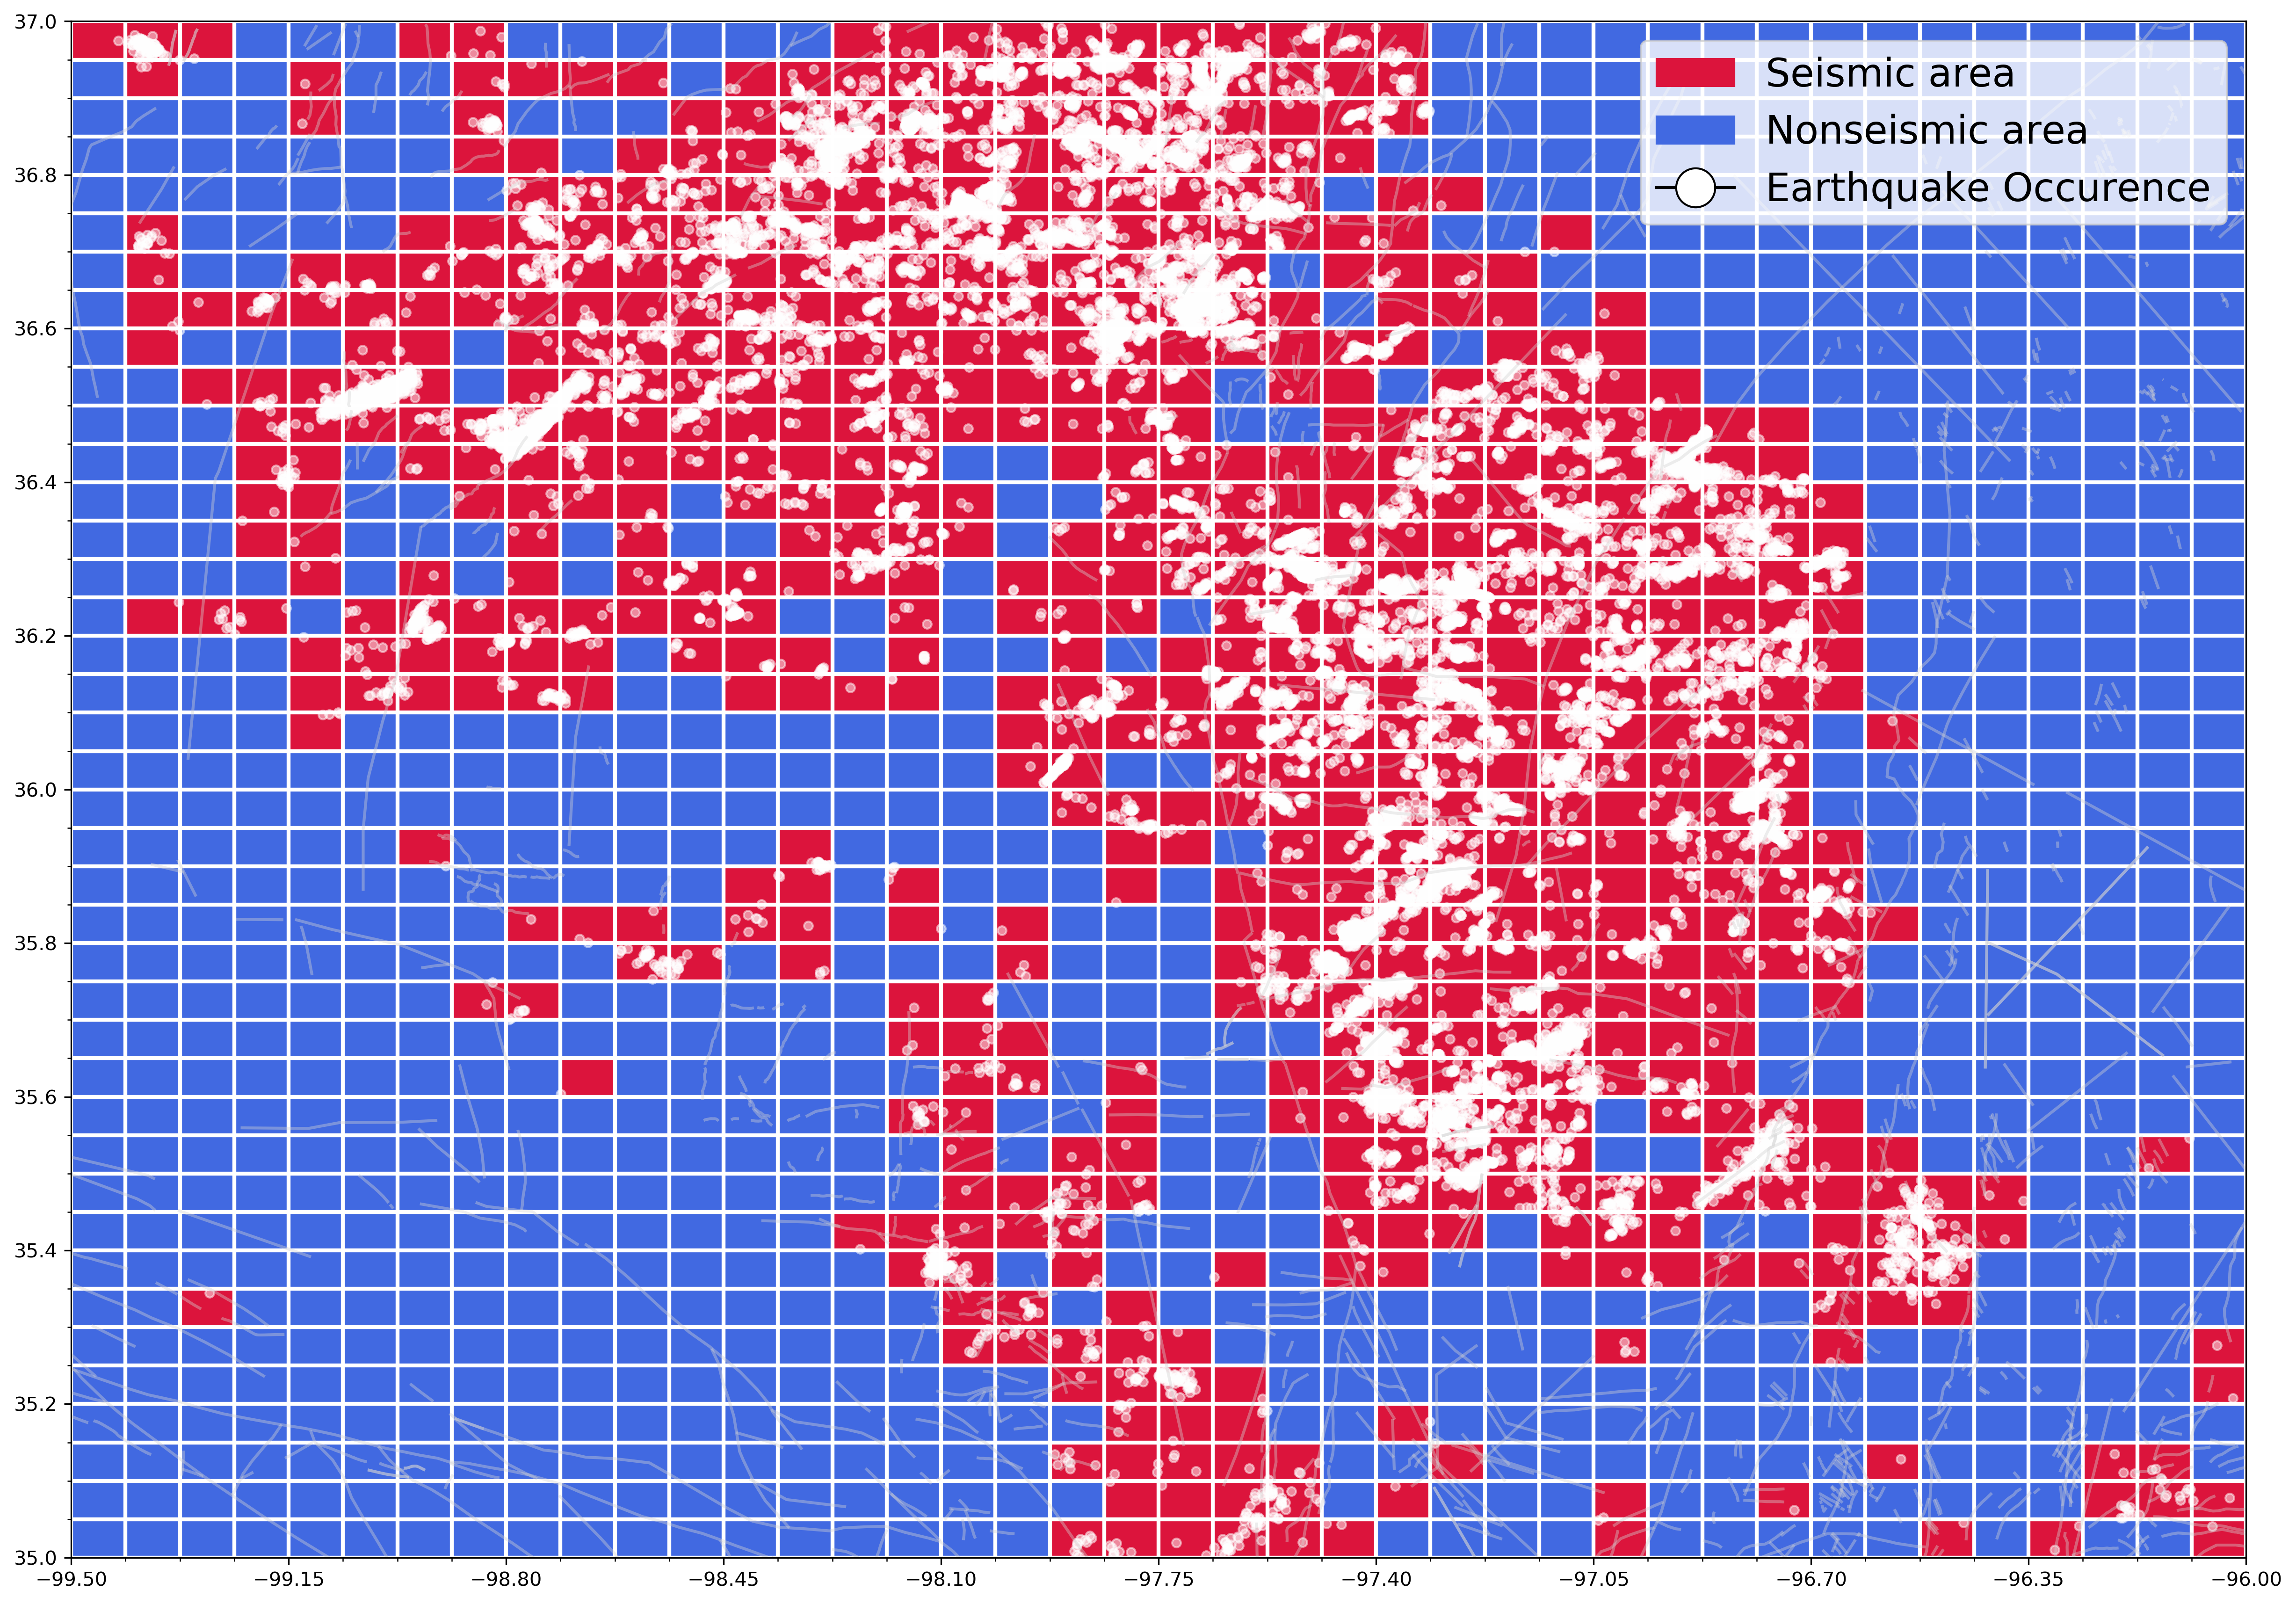
\includegraphics[width=1\textwidth]{target_mapping.png}
    \end{center}
    \caption{\label{fig:target_mapping} Target variable of earthquake occurrence within the interest area in Oklahoma.}
\end{figure}
After this statistical process, we obtained a dataset in terms of spatial distribution, each of which represents a subarea of our interest area and contains the values of features.
The target variable was based on seismicity, which represents the earthquake occurrence in spatial distribution, we assigned each grid a value of \textit{one} if there was at least one (magnitude\textgreater2) earthquake occurred during 2011 to 2018. 
Otherwise, if no earthquake occurred in this grid, we assigned it a value of \textit{zero}. The result grid of the earthquake occurrence (target) from 2011 to 2018 is shown in Figure~\ref{fig:target_mapping}. 
The white lines show the grid, with a spacing in the x direction of 8 km and the y direction of 5.5 km. The white points denotes the earthquake occurrences.
The red region denotes it has seismicity in this region and blue region denotes it does not have seismicity in this region. In our target grid, 42.5\% of the 1600 gird points are assigned the value '1'.

\subsection{Stepwise Feature Selection Approach}
\label{sec:SFSA}


As some activities are strongly overlapped in spatial distribution, they may have a high degree of multicollinearity. 
We calculated the feature similarity on all fearures based on Peason correlation coffecients and generated a heatmap as Figure~\ref{fig:heatmap}.
In general, We consider a high degree of collinearity between two features with a coefficient greater than 0.9, like 'active\_well\_number' and 'well\_under\_basement\_number'.
Therefore, in the process of selecting statistically significant features, we should also account for the high multicollinearity to prevent the influence in Section~\ref{sec:stepwise}.

To select 'best' features and deal with high multicollinearity problem, we use a forward stepwise approach introduced in Section~\ref{sec:stepwise}. We iteratively add a feature whilst ensuring the p-value of all current added feature remains below 0.05. 
This means that each feature we kept is statistically significant at the 95\% confidence level. Meanwhile, in each iteration step, we also deal with the high multicollinearity by checking the Variance Inflation Factor (VIF) for current kept features.
We iteratively eliminated the feature whose VIf is greater than 10 after adding a new feature (generally we think think there exists a high multicollinearity when VIF of some feature \textgreater 10).

\begin{figure}
    \begin{center}
        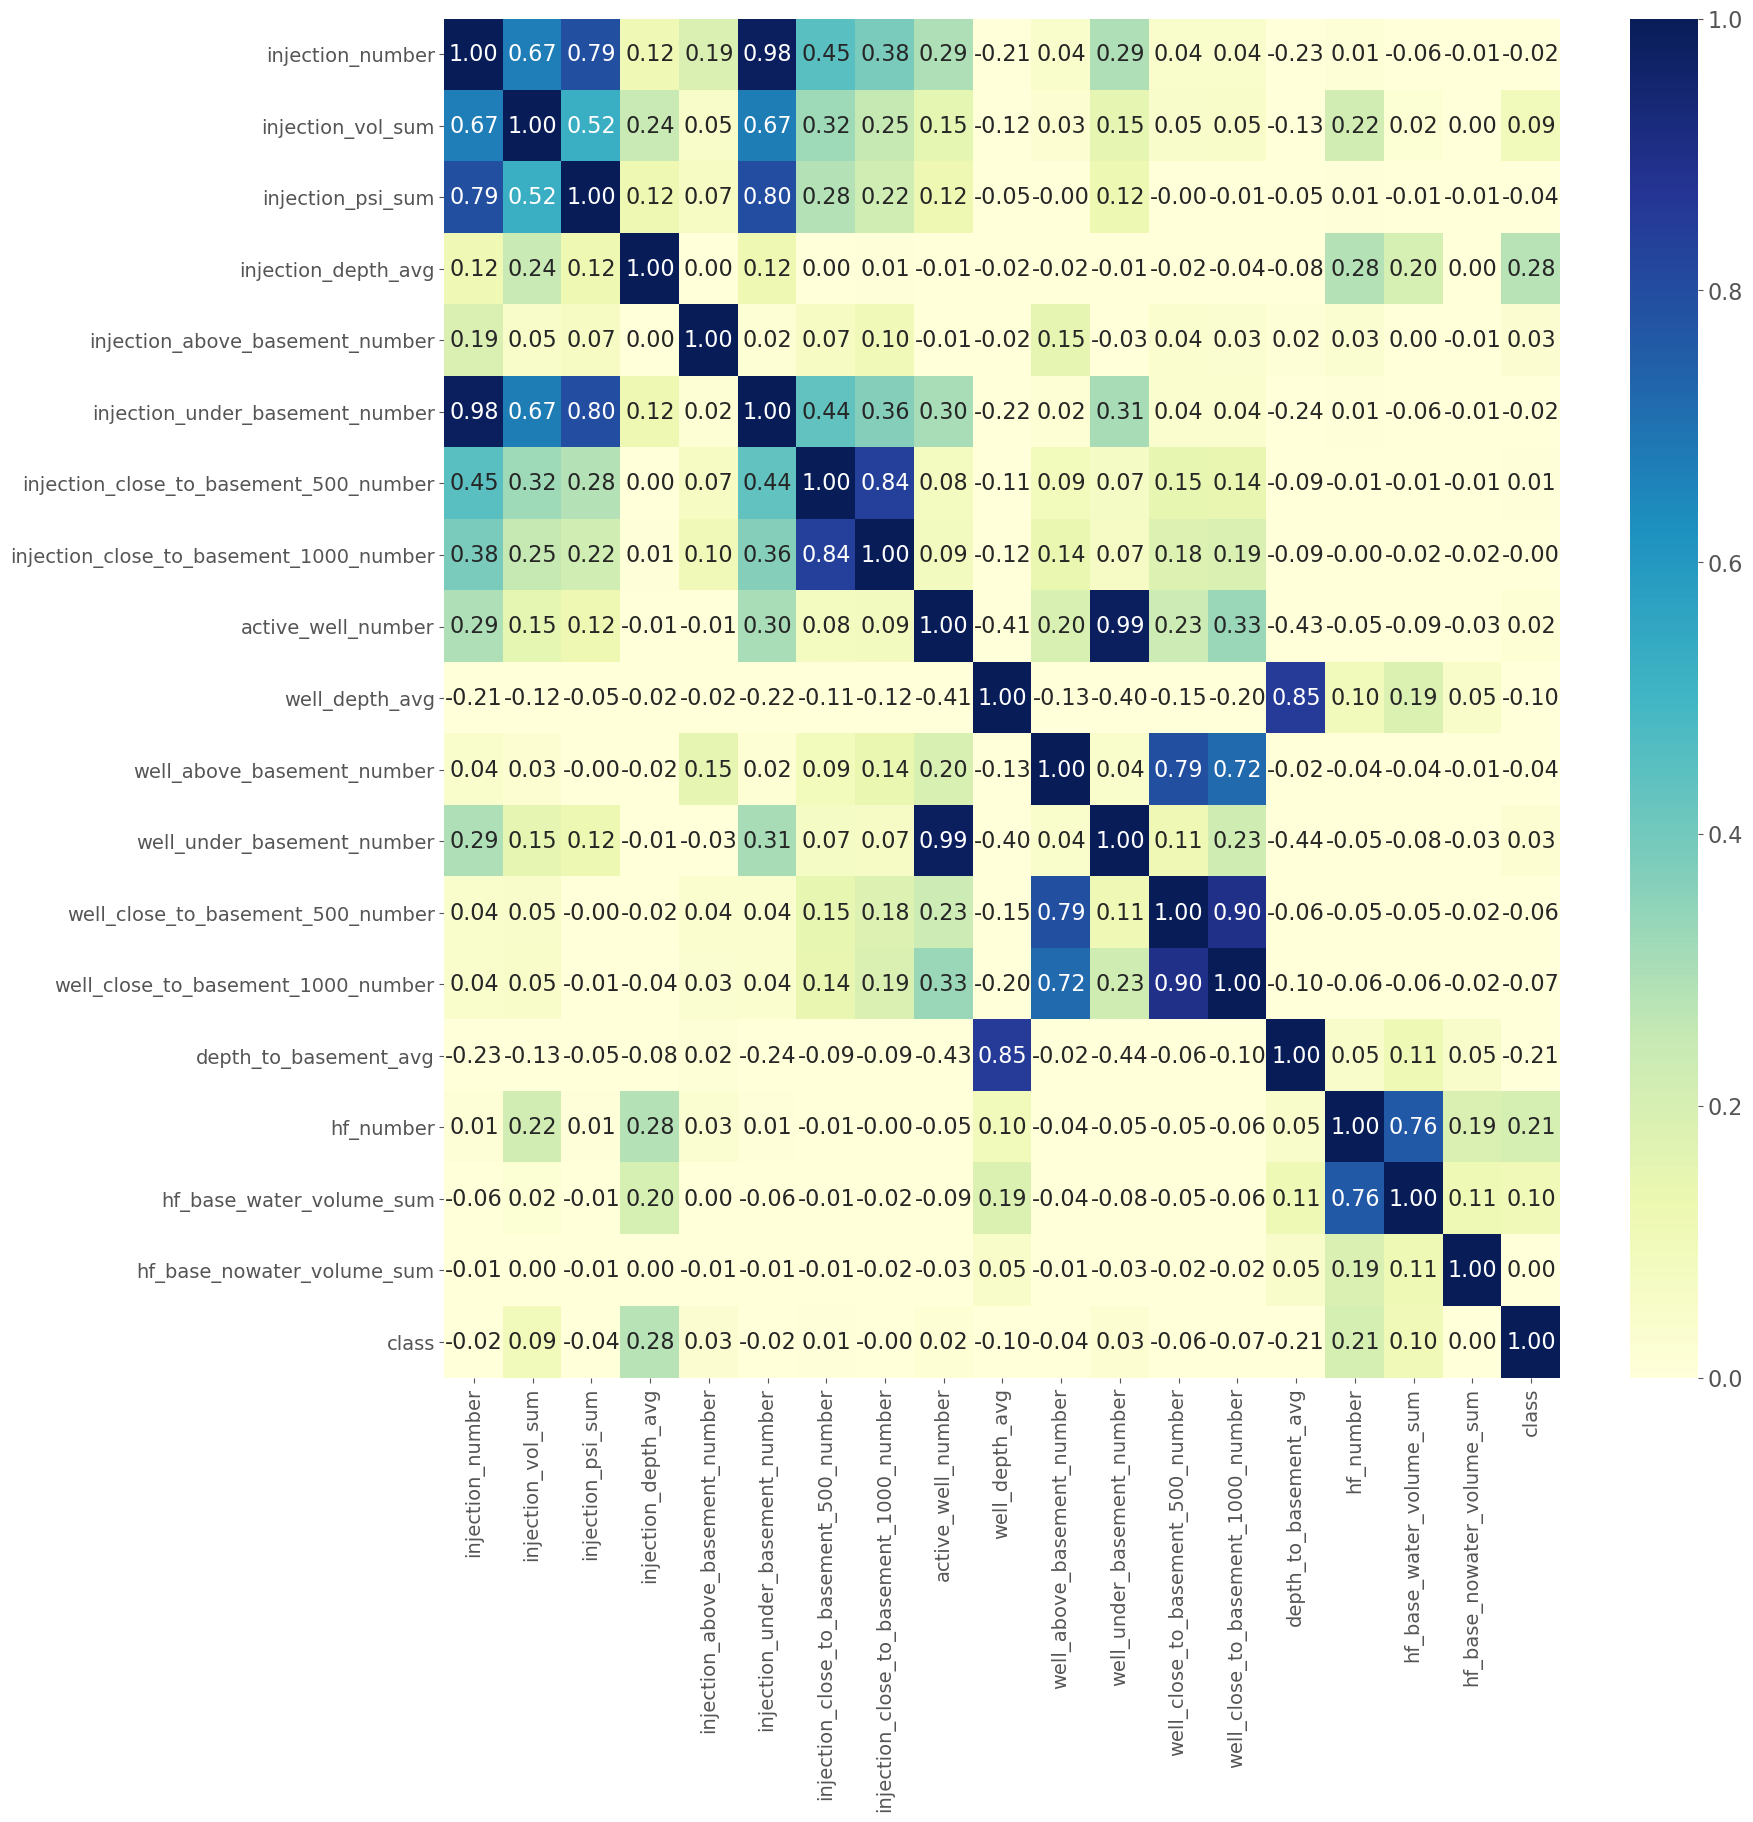
\includegraphics[width=0.8\textwidth]{heatmap_all.png}
    \end{center}
    \caption{\label{fig:heatmap} Correlation Heatmap.}
\end{figure}

After this process, we eliminated insignificant features and also solved the problem of high multicollinearity between variables. 
The result of features selecting with stepwise approach is shown in Figure~\ref{fig:stepwise}. 

\subsection{Logistic Regression Model}
\label{sec:LRM}
With the selected features in Section~\ref{sec:SFSA}, we constructed a multiple logistic regression model in this part. which used the features selected as independent variables (hf\_base\_water\_volume\_sum, hf\_number, depth\_to\_basement\_avg, well\_depth\_avd, injection\_under\_basement\_number, injection\_depth\_avg, injection\_vol\_sum) and earthquake occurrence as the target variable.
We standardise and normalise all input features by z-score normalization \citep{patro2015normalization} to reduce data skewness and bring all features on the same scale. The normalization of features allows us to interpret the relative difference in the model coffecients.

We splitted the dataset into train dataset and test dataset with the ratio of 9:1 , which have 1440 and 160 samples (Each sample is associated with one gird point in the interest area). In this build part, we use \textit{sklearn.linear\_model.LogisticRegression} to construct and fit our logistic model, which achieved the accuracy of 72.5\% on the test dataset.
The core part of code is shown in below:
\begin{lstlisting}[language=Python]
    X_train,X_test,y_train,y_test = train_test_split(X,Y,train_size=0.9, random_state=42)
    model = LogisticRegression()
    model.fit(X_train,y_train)
    model.score(X_test,y_test)
\end{lstlisting}
After fitting the model and testing, we check the coffecients for all input features by \textit{model.coef\_[0]} and plot them in Figure~\ref{fig:logistic_coffecients}. With the trained logistic model, we used the whole dataset to predict and compared output labels with true labels, which is shown in Figure~\ref{fig:logistic_result}.

\subsection{Neural Network Model}
\label{sec:NNM}
Due to the relatived low accuracy of prediction by logistic regression model in Section~\ref{sec:SFSA}, we used the neural network model to improve the accuracy of prediction, which can be used in practical. 
Because logistic regression is so simple that it is difficult to model for nonlinear data or data with polunomial correlation, it is hard to deal with the complicated problem. 
After all, in practice we don't know the actual relationship between earthquakes and these potential factors.
We don't even know if the relationship between input features and the target variable (earthquake occurrence) is linear or non-linear.
Therefore, neural network algorithm is suitable for the prediction of this kind of complicated problem. Neural network model have the ability to capture information contained in large amounts of data and build incredibly complex models. With the abilities of self-learning and high-speed for optimal solution, it easily achieves a higher performance compared with regression method.

\subsubsection{Architecture}
In this project, we use a neural network model which has its input layer with 7 neurons, two hidden layers of 8 neurons per layer and an outout layer with 2 neurons as shown in Figure~\ref{fig:neural_network_model}. 
In general, 1-5 hidden layers will serve for most problems and using the same number of neurons for all hidden layers will suffice. 
Therefore in this project, we choose to use two hidden layers and each layer has 8 neurons.
The input features used are also based on the feature selecting result in Section~\ref{sec:stepwise}, so we had seven input features for our training model.
It's taken for granted that we set the number of neurons to 7, which presents the each input feature.
For the earthquake prediction problem, which is a binary classification, so we use two neurons in output layer which one output neuron per positive class. The output represents the probability of the positive class (earthquake or no earthquake). We use the softmax activation function on the output layer to ensure the final probabilites sum to 1.


\subsubsection{Configuration}
For this prediction problem is classification problem, we use the cross-entropy \citep{de2005tutorial} as the loss function which serves well.
By lots of training attempts, we final used a set of hyperparameters which make the model performance in a well level.
Generally the best preformance is obtained by mini-batch sizes between 2 and 32, in training attempts, we found that the model performed best when the batch size was set to 16.
For the epoch size, we started from a large number of epochs and use early stopping to halt training when performance stops improving.
The selection of the learning rate is very important, we start with a very low value ($10^{-6}$) and slowly multiply it by a constant unitl it reaches a pretty high value (here the max value is 10).
We measured the performance (vs the log of learning rate) in \textit{Weights and Biases} to determine which rate served well for our earthquake prediction problem. We found $10^{-2}$ is best and we then retrrin our model using this optimal learning rate.
For the optimizer used in our model, we decide use Adam optimizer, which tends to be quite forgiving to a bad learning late and other non-optimal hyperparameters compared with most common used SGD optimizer.

The configuration which is called hyperparameters in machine learning is summarized below:

\begin{itemize}
    \item \textit{learning rate}: $10^{-2}$
    \item \textit{batch size}: 16
    \item \textit{epoch}: 200
    \item \textit{optimizer}: Adam
    \item \textit{loss function}: cross entropy
\end{itemize}

\begin{figure}
    \begin{center}
        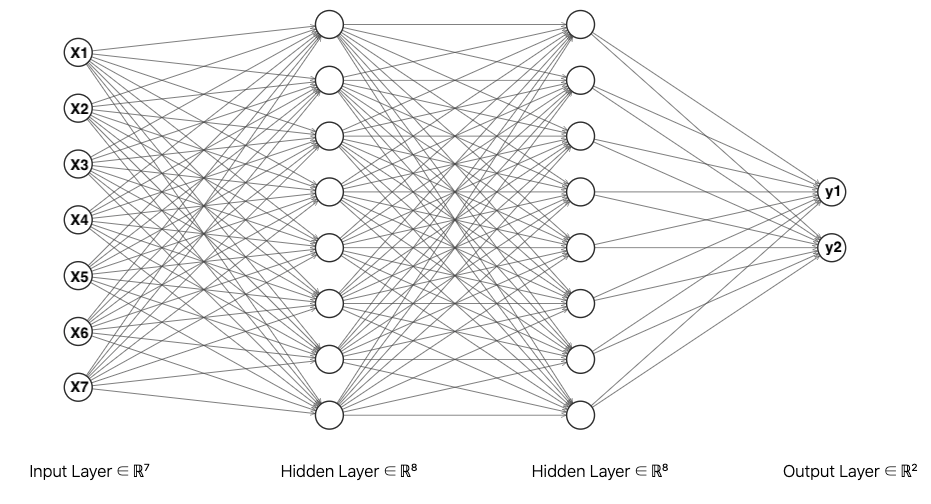
\includegraphics[width=1\textwidth]{neural_network_model.png}
    \end{center}
    \caption{\label{fig:neural_network_model} Neural Network Model Architecture.}
\end{figure}

\subsubsection{Training}
We initially divided the dataset into training dataset and testing dataset and normalised them as we done before fitting logistic regression model in \ref{sec:LRM}.
We use the Pytorch to conveniently generate the neural network model corresponding to architecture in Figure~\ref{fig:neural_network_model} by the code below:

\begin{lstlisting}[language=Python]
    class Net(nn.Module):
    def __init__(self,n_input, n_output):
        super(Net,self).__init__()
        self.linear1 = nn.Linear(n_input, 8)
        self.sigmoid1 = nn.Sigmoid()
        self.linear2 = nn.Linear(8, 8)
        self.sigmoid2 = nn.Sigmoid()
        self.linear3 = nn.Linear(8, n_output)

    def forward(self, x):
        lin1_out = self.linear1(x)
        sigmoid_out1 = self.sigmoid1(lin1_out)
        sigmoid_out2 = self.sigmoid2(self.linear2(sigmoid_out1))
        return self.linear3(sigmoid_out2)
\end{lstlisting}
As same with the Figure~\ref{fig:neural_network_model} shows, we implemented three linear transformations, which represents input layer to first hidden layer, first hidden layer to second hidden layer and second hidden layer to output layer.
Each transformation applies a linear transformation to the incoming data: $y = xA^{T} + b$. x represents the vector of neuron values before transformation and y represents a vector of neuron values after transformation.
A represents the weights multiplied in linear transformation (similar to coefficients in regression) and b represents the vector of bias. 
Our input layer corresponding to input features so we set the \textit{n\_input} variable in code to 7. 
Our output layer corresponding to output target class so we set the \textit{n\_output} variable in code to 2.
The \textit{\_\_init\_\_} function defines the architecture of neural network. The \textit{forward} function in the code represents the process of propagation.

we trained the model by 200 epochs in total. For each epoch, we trained by the whole training dataset and test the accuracy of current model in testing dataset.  We used \textit{torch.utils.data.DataLoader} to load the training dataset and testing dataset.
Then, everytime we load a batch (16 samples) of training data and input into model for prapagation, then the outputs were compared with the labels. According to loss of current batch, we updated the weights in model by \textit{optimizer.step()}.
After training by one epoch, we calculate the accuracy of model in whole training dataset and whole testing dataset and updated the loss value in log plot. The training performance figure of our model is shown in Figure~\ref{fig:training_process}.
By use the network model trained, we achieved a much better accuracy of 80.6\% on testing dataset compared with logistic regression model in Section~\ref{sec:LRM}.
Similarly, we also used the whole dataset to predict by our trained neural network model and compared output labels with true labels, which is shown in Figure~\ref{fig:neural_network_result}.

\section{Results and Discussion}
This section will analogize the results from Section~\ref{sec:Implementation}.

\subsection{Visualiztion}

\begin{figure}
    \begin{center}
        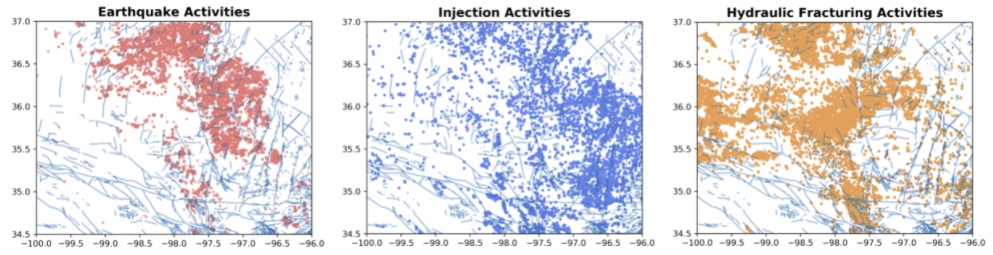
\includegraphics[width=1\textwidth]{activity.png}
    \end{center}
    \caption{\label{fig:activity} Activities during 2011 to 2018 in interest area from Oklahoma.}
\end{figure}

\begin{figure}
    \begin{center}
        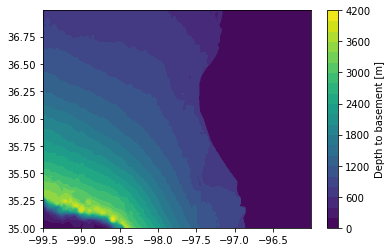
\includegraphics[width=0.6\textwidth]{depth_to_basement.png}
    \end{center}
    \caption{\label{fig:depth_to_basement} Depth to basement in Oklahoma.}
\end{figure}

Through these activities distribution in Fig~\ref{fig:activity} and Fig~\ref{fig:depth_to_basement}, we can found a rough spatial correlation between some of them.
We firstly compared the depth to basement with earthquake activities, we found the lower left region of interest area has a thicker softer sedimentary rocks than upper right region (In the Figure~\ref{fig:depth_to_basement} it showes lower left region has larger depth value and upper right region almost has 0 value).
It is can be inferred that the induced seismicity may be related to depth to basement. 
Besides, the injection activities are similar to earthquakes activities in spatial distribution. 
As the Figure~\ref{fig:activity} shows, the three black rectangular regions (marked by 1 to 3) represents the activities dense area, which are highly similar in spatial distribution, even in small area as rectangular area 3. 
By the high similarity, we can concluded that the induced seismicity have high correlation with injection activities.
For the hydraulic fracturing activities and well spatial data, we can not found some relation beteen induced earthquake and them and we need to explore and interpret through the model generated.

\subsection{Stepwise Approach}
The Process of features selection with stepwise approach is shown in below block and the feature result along with their p-value and VIF are shown in Figure~\ref{fig:stepwise}.

\begin{figure}
    \begin{center}
        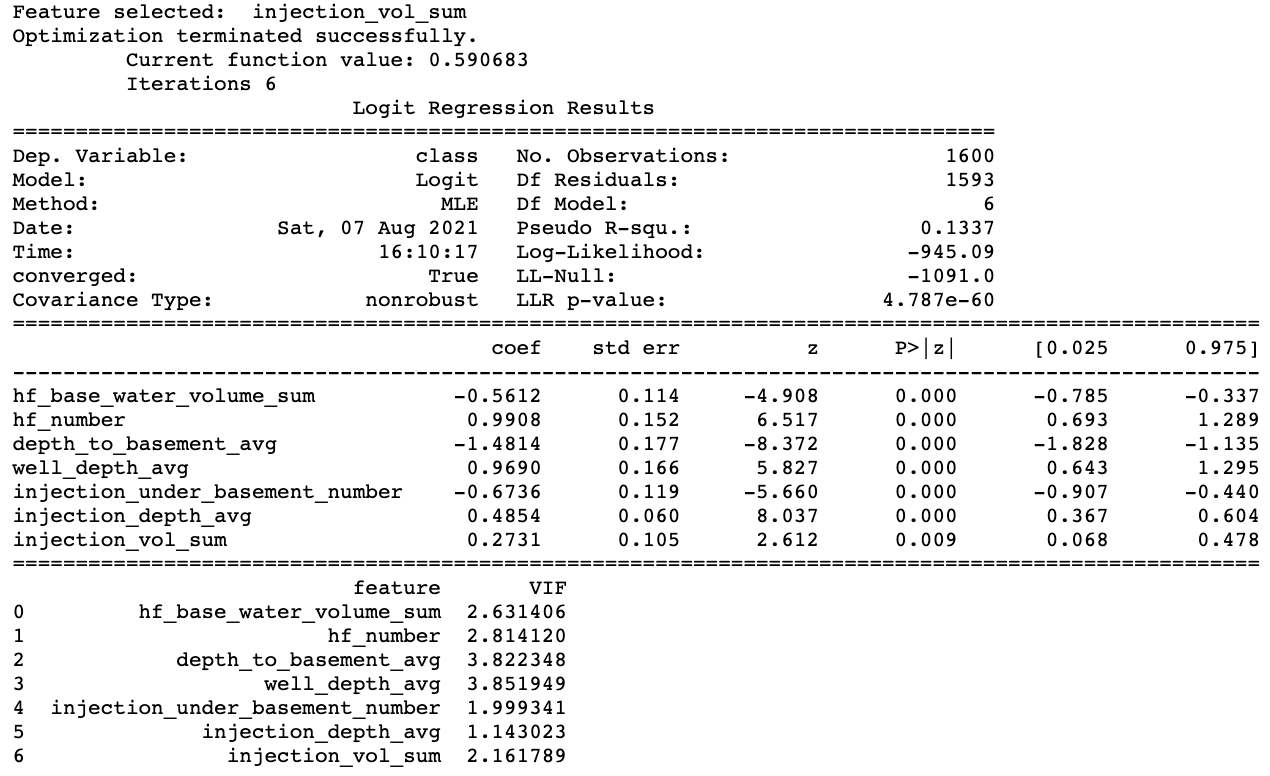
\includegraphics[width=1\textwidth]{stepwise.png}
    \end{center}
    \caption{\label{fig:stepwise} Feature Selection Result with Stepwise Approach.}
\end{figure}

\begin{itemize}
\item Iteration 1\\
Feature selected: hf\_base\_nowater\_volume\_sum\\
P-value \textgreater 0.05 check: hf\_base\_nowater\_volume\_sum\\
Feature removed: hf\_base\_nowater\_volume\_sum\\
VIF\textgreater 10 check: None\\
Feature removed: None

\item Iteration 2\\
Feature selected: hf\_base\_water\_volume\_sum\\
P-value \textgreater 0.05 check: None\\
VIF\textgreater 10 check: None\\
Feature removed: None\\

\item Iteration 3\\
Feature selected: hf\_number\\
P-value \textgreater 0.05 check: None\\
VIF\textgreater 10 check: None\\
Feature removed: None\\

\item Iteration 4\\
Feature selected: depth\_to\_basement\_avg\\
P-value \textgreater 0.05 check: None\\
VIF\textgreater 10 check: None\\
Feature removed: None\\

\item Iteration 5\\
Feature selected: well\_under\_basement\_number\\
P-value \textgreater 0.05 check: None\\
VIF\textgreater 10 check: None\\
Feature removed: None\\

\item Iteration 5\\
Feature selected: well\_depth\_avg\\
P-value \textgreater 0.05 check: None\\
VIF\textgreater 10 check: None\\
Feature removed: None\\

\item Iteration 6\\
Feature selected: active\_well\_number\\
P-value \textgreater 0.05 check:  well\_under\_basement\_number(0.477), active\_well\_number(0.772)\\
Feature removed: active\_well\_number\\
VIF\textgreater 10 check: None\\
Feature removed: None\\

\item Iteration 7\\
Feature selected: injection\_under\_basement\_number\\
P-value \textgreater 0.05 check: well\_under\_basement\_number(0.102)\\
Feature removed: well\_under\_basement\_number\\
VIF\textgreater 10 check: None\\
Feature removed: None\\

\item Iteration 8\\
Feature selected: injection\_depth\_avg\\
P-value \textgreater 0.05 check: None\\
Feature removed: None\\
VIF\textgreater 10 check: None\\
Feature removed: None\\

\item Iteration 9\\
Feature selected: injection\_psi\_sum\\
P-value \textgreater 0.05 check: injection\_psi\_sum(0.969)\\
Feature removed: injection\_psi\_sum\\
VIF\textgreater 10 check: None\\
Feature removed: None\\

\item Iteration 10\\
Feature selected: injection\_vol\_sum\\
P-value \textgreater 0.05 check: None\\
Feature removed: None\\
VIF\textgreater 10 check: None\\
Feature removed: None\\
\end{itemize}

We can see all the selected features by stepwise approach meet the requirement of p-value \textless 0.05 and VIF \textless 10.
This means we successfully eliminated the features which are not statistically significant and there is no high multicollinearity in all features selected.  

\subsection{Model Comparison}
\subsubsection{Logistic Regression Model}
By the Section~\ref{sec:LRM} and Section~\ref{sec:NNM}, we fitting the logistic regression model and training the configured neural network model on the training dataset, 
the prediction accuracy on testing dataset for these two models achieves at 72.18\% and 77.5\% respectively. This denotes that neural netwok model performs better than logistic regression model.
Besides, we extraly use these models to test on the whole dataset, which contains all the grids point of interpret area.
The Indicators which we usually used to assess for models in machine learning field are calculated and listed in Table~\ref{tab:Indicators}.

% Please add the following required packages to your document preamble:
% \usepackage{graphicx}
\begin{table}[]
    \centering
    \caption{Indicators of two modules}
    \label{tab:Indicators}
    \begin{tabular}{|c|c|c|c|c|}
    \hline
    Model\textbackslash{}Indicator & ACC   & Precision & Recall & F1-score \\ \hline
    Logistic Regression Model      & 0.705 & 0.705     & 0.530  & 0.604    \\ \hline
    Neural Network Model           & 0.79  & 0.734     & 0.792  & 0.762    \\ \hline
    \end{tabular}
    \end{table}
The \textit{ACC} refers to accuracy, which denotes the proportion of all correct predictions in the total predictions. 
We can see for all regions in interpret area, the prediction accuracy of NN model is 10 percent higher than LR model.
The \textit{ACC} is a simple indictor in model evaluation, it is an inituitive representation of whether the model is capable of making accurate predictions.
However, it is easily affected by the imbalance of the samples. For example, there are a total of 100 samples and 90 of them are positive samples.
If the model predicts all samples to positive sample, the accuracy can reaches up to 90\%, but such a model is meaningless obviously.  
Fortunately, the samples in our dataset are relatively balanced, which have 680 positive samples and 920 negative samples in the ratio of 2:3 as shown in Figure~\ref{fig:class_label}.
Therefore, accuracy can be a import indictor for model comparison and evaluation in this project. 
Through the \textit{ACC} comparison for LR model and NN model in Table~\ref{tab:Indicators}, we can concluded that our NN model have a better ability pf prediction than LR model.

\begin{figure}
    \begin{center}
        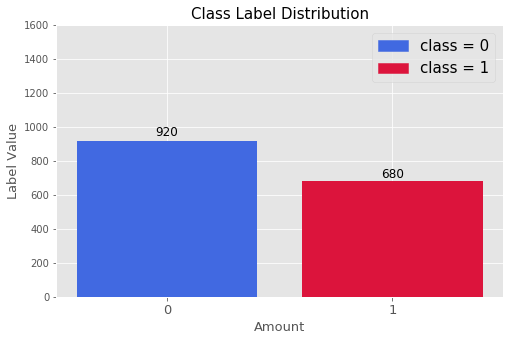
\includegraphics[width=0.7\textwidth]{class_label.png}
    \end{center}
    \caption{\label{fig:class_label} Class Label Distribution in whole dataset.}
\end{figure}

In a classification problem, precision attempts to answer the question that what proportion of positive identifications was actually correct. 
The Recall attempts to answer the question that what proportion of actual positives was identified correctly.

\begin{figure}
    \begin{center}
        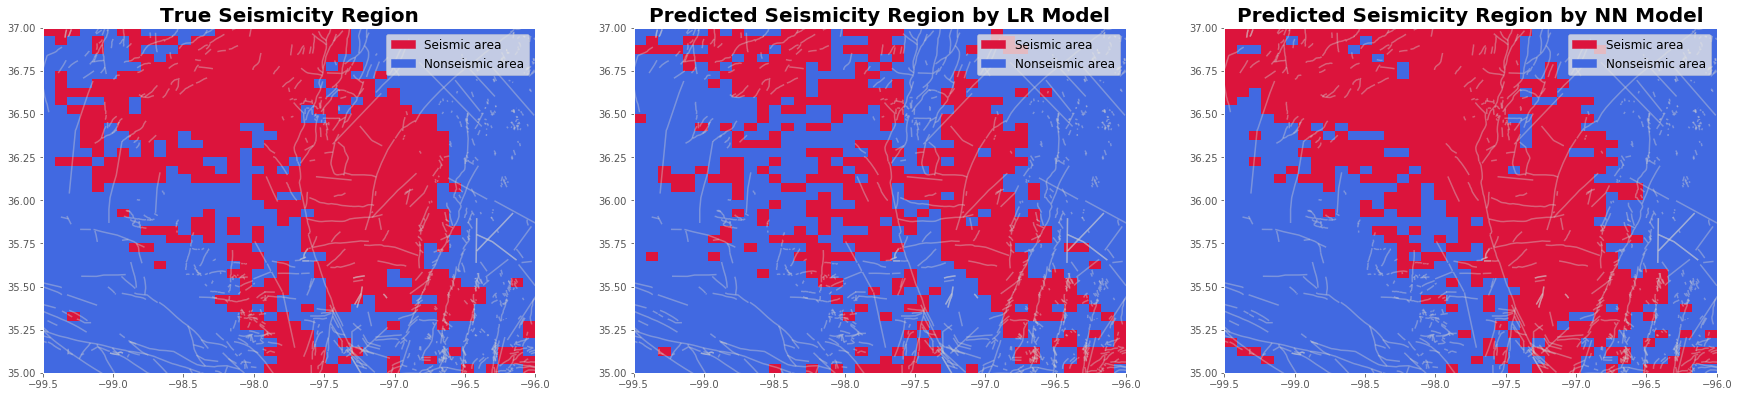
\includegraphics[width=1\textwidth]{mapping_comparison.png}
    \end{center}
    \caption{\label{fig:logistic_result} Seismicity Prediction by Logistic Regression Model and Neural Network Model.}
\end{figure}

The prediction accuracy achieved 70.75\% by the comparison between seismicity in truth and prediction.
Generally three dense regions distribution are correctlypredicted, but the precision of regional outline is pretty poor.

\begin{figure}
    \begin{center}
        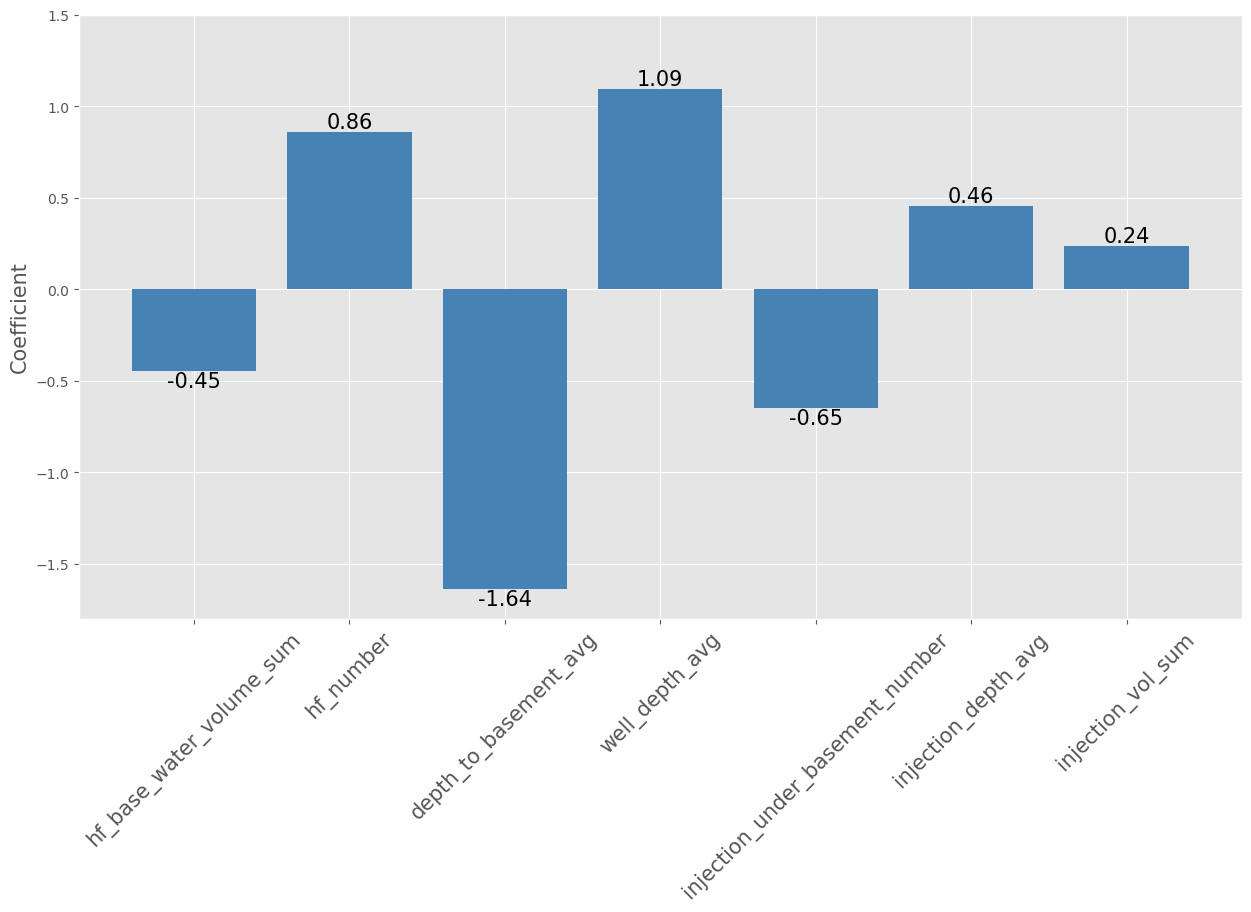
\includegraphics[width=1\textwidth]{logistic_coefficients.png}
    \end{center}
    \caption{\label{fig:logistic_coffecients} Coffecients for Features in Fitted Logistic Regression Model.}
\end{figure}

\begin{figure}
    \begin{center}
        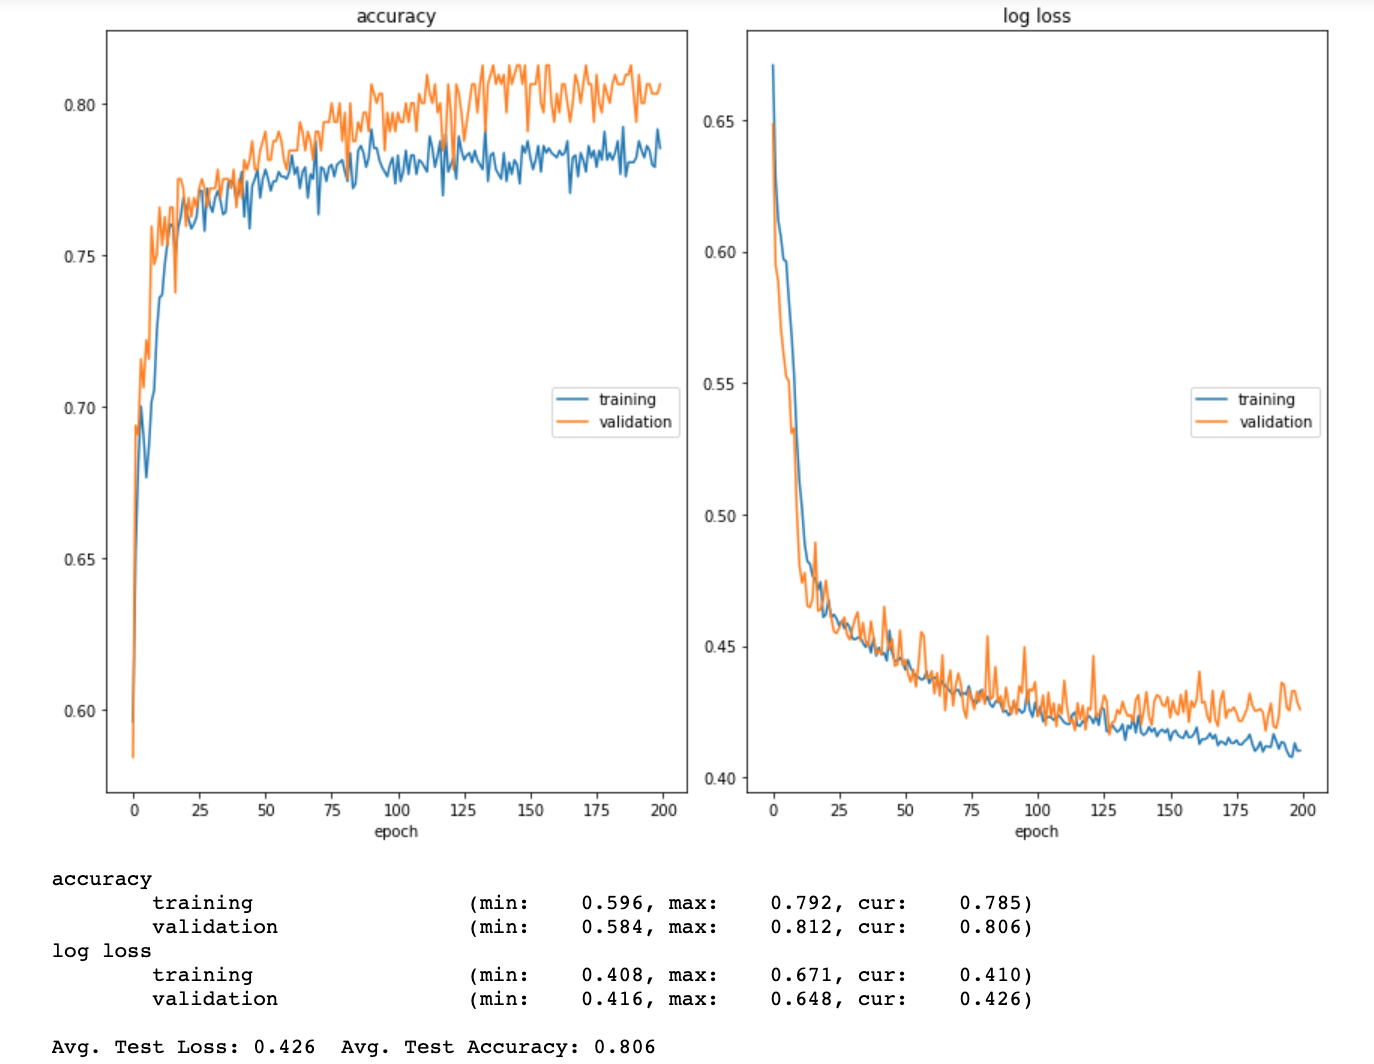
\includegraphics[width=1\textwidth]{training_process.png}
    \end{center}
    \caption{\label{fig:training_process} Neural Network Model Training Process.}
\end{figure}

\begin{figure}
    \begin{center}
        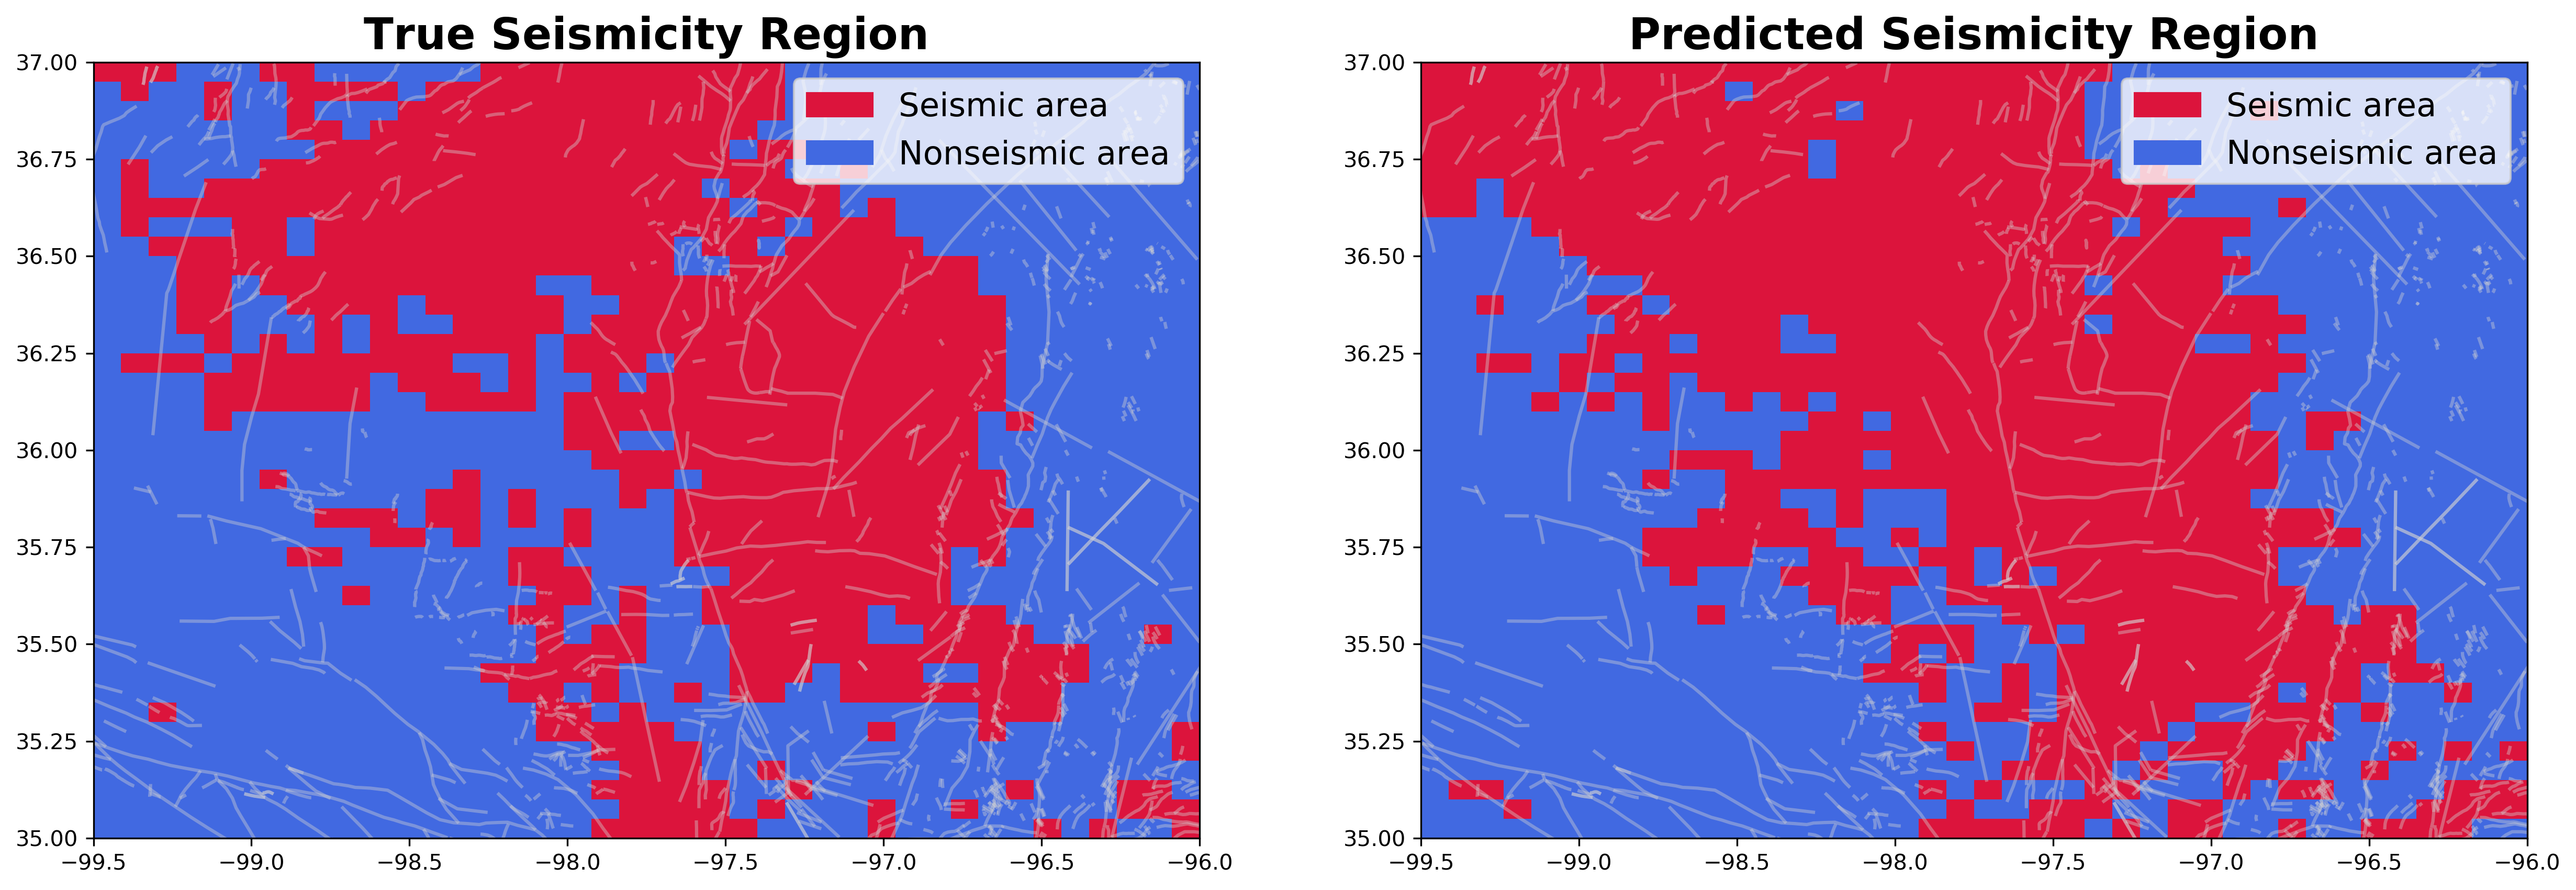
\includegraphics[width=1\textwidth]{neural_network_result.png}
    \end{center}
    \caption{\label{fig:neural_network_result} Seismicity Prediction with Trained Neural Network Model.}
\end{figure}
\section{Conclusion and Future Work}





\newpage
% References
\bibliographystyle{agsm}
\bibliography{references.bib}  % BibTeX references are saved in references.bib
\section{Appendix}
\begin{figure}
    \begin{center}
        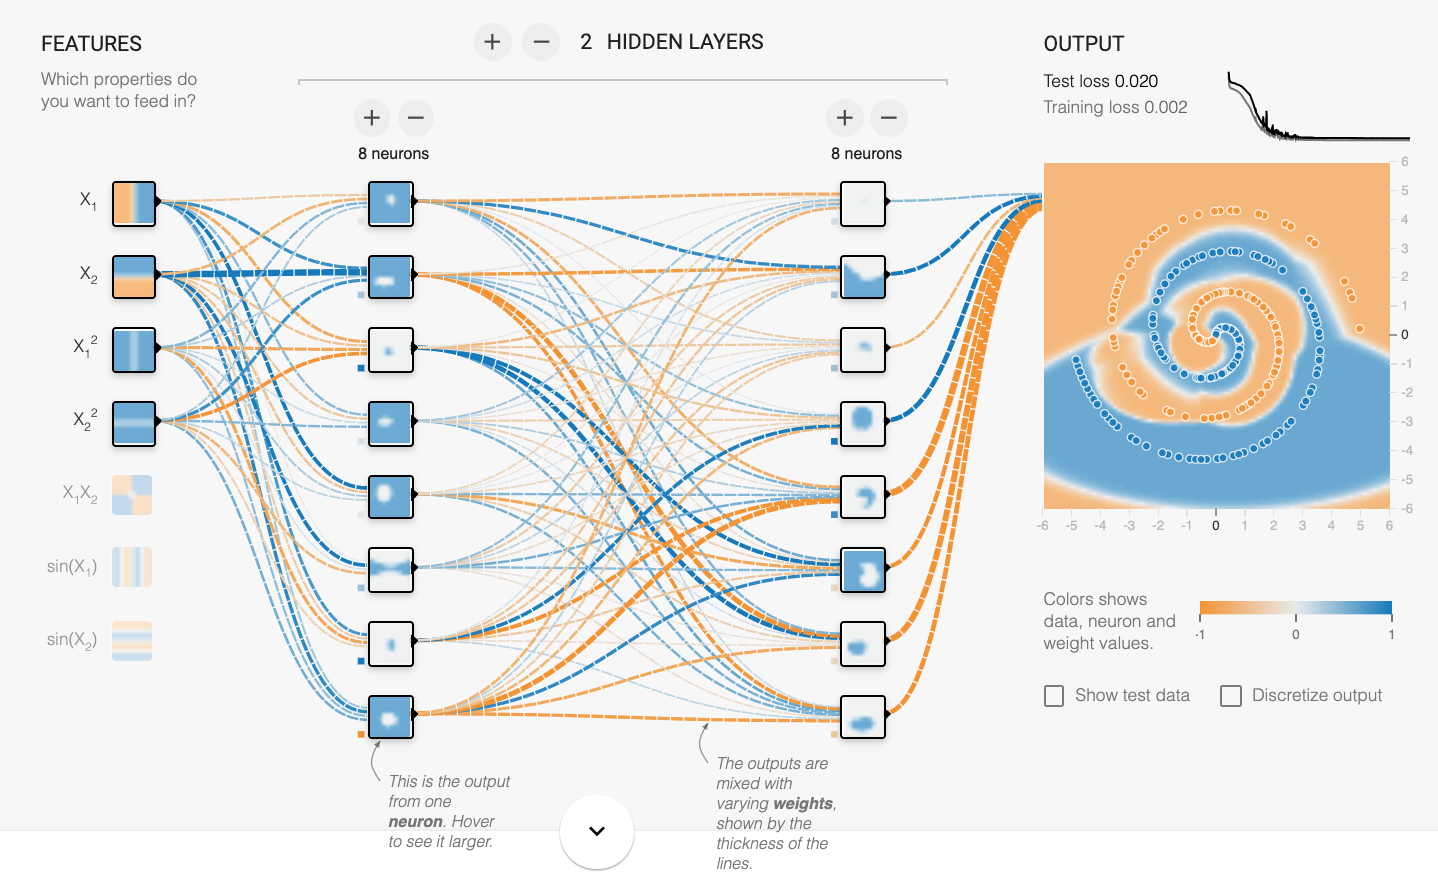
\includegraphics[width=1\textwidth]{neural_network_exmaple.png}
    \end{center}
    \caption{\label{fig:neural_network_example} The model created from above code simulated through playground.tensorflow.org}
\end{figure}

\begin{figure}
    \begin{center}
        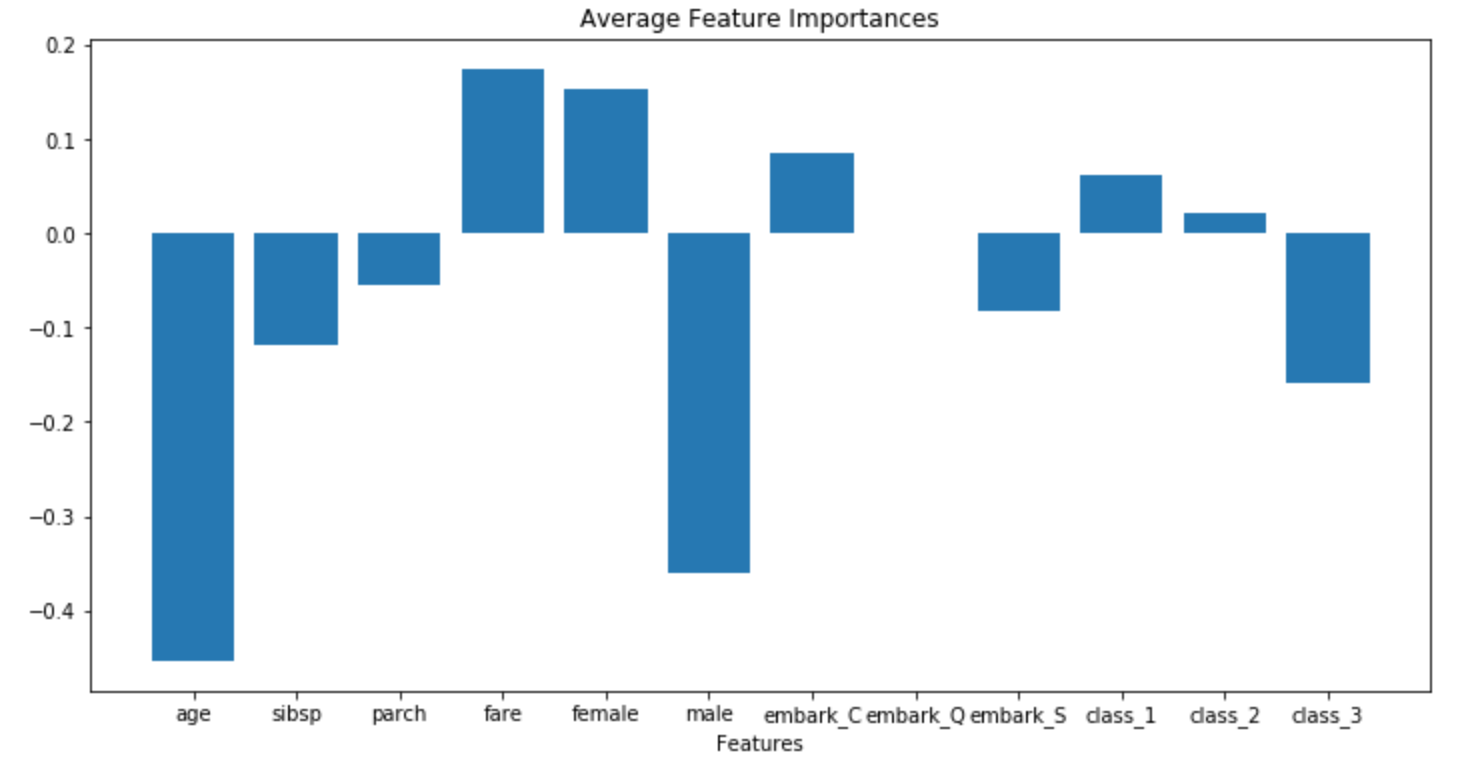
\includegraphics[width=0.8\textwidth]{feature_importance.png}
    \end{center}
    \caption{\label{fig:feature_importance} Feature Importance Example in Captum Tutorial.}
\end{figure}
\end{document}          

